\PassOptionsToPackage{export}{adjustbox}
\documentclass[
	11pt,
	aspectratio=169,
]{beamer}

\graphicspath{{supplement/}{./}}

\usepackage{booktabs}
\usepackage{multirow}
\usepackage{amsmath,amssymb,amsfonts}
\usepackage{algorithm}
\usepackage{algorithmic}
\usepackage{graphicx}
\usepackage{caption}
\usepackage{subcaption}
\usepackage{tikz}
\usetikzlibrary{shapes.geometric,arrows,positioning}
\usepackage{standalone}
\usepackage{colortbl}
\usepackage[export]{adjustbox} % For max width/height in includegraphics

% Global Image Constraints
\setkeys{Gin}{max width=0.9\textwidth, max height=0.75\textheight, keepaspectratio}

% Global List Spacing
\setbeamertemplate{itemize/enumerate body begin}{\small}
\setbeamertemplate{itemize/enumerate subbody begin}{\footnotesize}
\setlength{\leftmargini}{1.5em}
\setlength{\leftmarginii}{1.2em}
\setlength{\itemsep}{0.3em} 

% Theme
\usetheme{Boadilla}
\usecolortheme{seahorse}

% Custom Colors
\definecolor{mathblue}{RGB}{0,51,102}
\definecolor{mathgray}{RGB}{64,64,64}
\definecolor{lightgray}{RGB}{240,240,240}

\setbeamercolor{structure}{fg=mathblue}
\setbeamercolor{frametitle}{fg=mathblue,bg=white}
\setbeamercolor{title}{fg=mathblue}
\setbeamercolor{author}{fg=mathgray}

% Fonts
\usefonttheme{default}
\usepackage{palatino}
\usepackage[default]{opensans}

% Custom Frametitle
\let\oldframetitle\frametitle
\renewcommand{\frametitle}[1]{%
    \ifx\insertsection\empty%
        \oldframetitle{#1}%
    \else%
        \oldframetitle{%
            {\small\color{mathblue}\textbf{\thesection. \insertsection}}%
            \hspace{0.4em}{\color{gray!50}|}\hspace{0.4em}%
            #1%
        }%
    \fi%
}

\title[Attention Is All You...]{Attention Is All You Need}
\subtitle{Generated by Paper2PPT (github.com/gejifeng/Paper2PPT)}
\author{Ashish Vaswani, Noam Shazeer, Niki Parmar, Jakob Uszkoreit, Llion Jones, Aidan N. Gomez, Łukasz Kaiser, Illia Polosukhin}
\date{\today}

\begin{document}\begin{frame}
	\titlepage
\end{frame}
\begin{frame}{Overview}
	\tableofcontents
\end{frame}




\section{Introduction}



\begin{frame}{The Problem with Recurrence}
    \begin{block}{The Core Limitation of RNNs/LSTMs}
    Computation is \textbf{inherently sequential}. To compute hidden state $h_t$, you must first compute $h_{t-1}$.
\end{block}

\begin{itemize}
    \item \textbf{Prevents parallelization} within a training example.
    \item Training on long sequences becomes slow and memory-intensive.
    \item Limits effective batching due to memory constraints.
    \item This is the \textbf{fundamental constraint} the Transformer aims to solve.
\end{itemize}

\begin{block}{The Goal}
    A new architecture that is \textbf{more parallelizable} and requires \textbf{significantly less time to train} while maintaining or improving model quality.
\end{block}
\end{frame}
\begin{frame}{Attention as a Solution}
    \begin{block}{The Core Idea}
    The \textbf{Transformer} architecture dispenses with recurrence and convolution, relying \textbf{solely} on attention mechanisms for sequence transduction.
\end{block}

\begin{itemize}
    \item Attention mechanisms model dependencies \textbf{regardless of distance} in the sequence.
    \item This overcomes the \textbf{sequential bottleneck} of RNNs, enabling full parallelization.
    \item The model draws \textbf{global dependencies} between input and output in constant steps.
    \item It achieves superior translation quality with significantly \textbf{less training time}.
\end{itemize}
\end{frame}



\section{Background}



\begin{frame}{Prior Work \& Gaps}
    \begin{columns}[T,onlytextwidth]
    \begin{column}{0.48\textwidth}
        \begin{block}{Convolutional Approaches}
            \begin{itemize}
                \item ByteNet and ConvS2S used CNNs.
                \item Operations to relate distant positions grow with distance (linearly/logarithmically).
                \item This makes learning long-range dependencies difficult.
            \end{itemize}
        \end{block}
    \end{column}
    \begin{column}{0.48\textwidth}
        \begin{block}{The Self-Attention Concept}
            \begin{itemize}
                \item Relates different positions of a single sequence.
                \item Computes a representation using a weighted sum of all positions.
                \item Complexity is constant for any distance.
            \end{itemize}
        \end{block}
        \begin{alertblock}{Transformer's Novelty}
            First transduction model based \textbf{solely} on self-attention, without RNNs or convolutions.
        \end{alertblock}
    \end{column}
\end{columns}
\end{frame}



\section{Methodology}



\begin{frame}{Core Architecture}
\vspace{-0.5em}
\begin{columns}[c,onlytextwidth]
\begin{column}{0.6\textwidth}
    \begin{block}{Encoder-Decoder Architecture}
        The Transformer follows the standard encoder-decoder structure for sequence transduction.
    \end{block}
    \vspace{-0.5em}
    \begin{itemize}
        \setlength{\itemsep}{0pt}
        \item \textbf{Encoder}: Maps input sequence $(x_1, ..., x_n)$ to continuous representation $\mathbf{z}$.
        \item \textbf{Decoder}: Generates output sequence $(y_1, ..., y_m)$ autoregressively.
        \item \textbf{Auto-regressive}: At each step, decoder consumes previously generated symbols.
    \end{itemize}
    \vspace{-0.5em}
    \begin{block}{Key Innovation}
        Replaces recurrence and convolution with \textbf{stacked self-attention} and point-wise feed-forward layers.
    \end{block}
\end{column}
\begin{column}{0.38\textwidth}
    \centering
    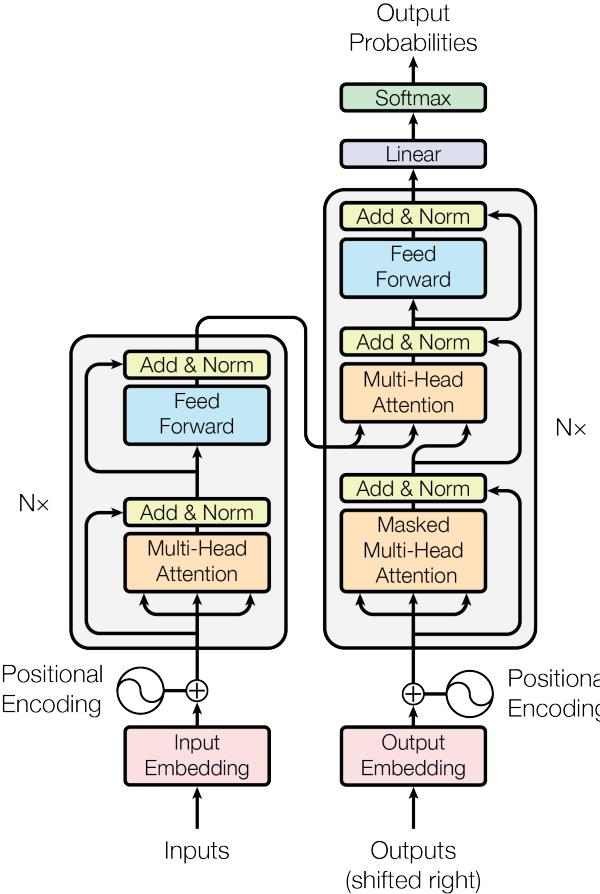
\includegraphics[width=\linewidth, height=0.75\textheight, keepaspectratio]{supplement/ee461f4421b4b3ee9ee47f2df3147cd6c5ea8ecec38495a9b419497230cdc1a3.jpg}
    \small
    Figure 1: Transformer model architecture.
\end{column}
\end{columns}
\end{frame}
\begin{frame}{Scaled Dot-Product Attention}
    \centering
\begin{alertblock}{Scaled Dot-Product Attention}
    \begin{equation*}
        \mathrm{Attention}(Q, K, V) = \mathrm{softmax}\left(\frac{QK^{T}}{\sqrt{d_k}}\right)V
    \end{equation*}
\end{alertblock}

\begin{block}{Purpose of Scaling}
    Scaling by \(1 / \sqrt{d_k}\) prevents large dot products that push the softmax into regions with extremely small gradients.
\end{block}
\end{frame}
\begin{frame}{Multi-Head Attention}
\begin{adjustbox}{max totalheight=0.90\textheight, keepaspectratio, center}
\begin{minipage}{\linewidth}
\begin{columns}[c,onlytextwidth]
\begin{column}{0.38\textwidth}
    \centering
    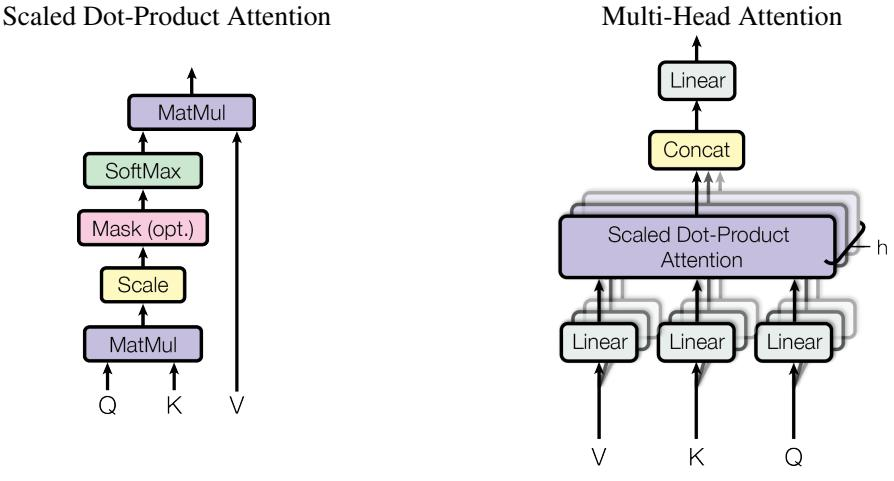
\includegraphics[width=\linewidth, height=0.8\textheight, keepaspectratio]{supplement/0156f05989374f32a550354bccdcbf7ea80a5a1aa98f2cf1572da70c5d319e4d.jpg}
\end{column}
\begin{column}{0.6\textwidth}
    \begin{block}{Motivation}
        Single-head attention averages across the full representation space. Multi-head attention allows the model to \textbf{jointly attend to information from different representation subspaces} at different positions.
    \end{block}
    \vspace{-0.5em}
    \begin{block}{Multi-Head Attention}
        \begin{equation*}
            \begin{aligned}
            \mathrm{MultiHead}(Q,K,V) &= \mathrm{Concat}(\mathrm{head}_1, ..., \mathrm{head}_h)W^O \\
            \text{where } \mathrm{head}_i &= \mathrm{Attention}(QW_i^Q, KW_i^K, VW_i^V)
            \end{aligned}
        \end{equation*}
    \end{block}
    \vspace{-0.5em}
    \begin{itemize}
        \setlength{\itemsep}{0pt}
        \item Uses $h$ parallel attention ``heads''.
        \item Each head has its own learned linear projections.
        \item Standard config: $h = 8$ heads.
        \item With $d_{\text{model}}=512$, $d_k = d_v = d_{\text{model}} / h = 64$.
    \end{itemize}
\end{column}
\end{columns}
\end{minipage}
\end{adjustbox}
\end{frame}
\begin{frame}{Three Uses of Attention}
    \begin{footnotesize}
\begin{columns}[T,onlytextwidth]
    \begin{column}{0.32\textwidth}
        \textbf{Encoder Self-Attention}
        \begin{itemize}
            \item Keys, values, queries from \textbf{same} encoder layer.
            \item Each position attends to \textbf{all positions} in the previous layer.
            \item Computes a representation of the full input sequence.
        \end{itemize}
    \end{column}
    \begin{column}{0.32\textwidth}
        \textbf{Decoder Masked Self-Attention}
        \begin{itemize}
            \item Keys, values, queries from \textbf{same} decoder layer.
            \item Each position attends only to \textbf{earlier positions} (masked).
            \item Preserves the auto-regressive property during generation.
        \end{itemize}
    \end{column}
    \begin{column}{0.32\textwidth}
        \textbf{Encoder-Decoder Attention}
        \begin{itemize}
            \item Queries from \textbf{decoder}; keys/values from \textbf{encoder} output.
            \item Lets decoder attend to \textbf{relevant parts} of the input sequence.
            \item Mimics classic seq2seq attention mechanisms.
        \end{itemize}
    \end{column}
\end{columns}
\end{footnotesize}

\begin{block}{Core Principle}
All three are instances of \textbf{Multi-Head Attention}. The function is the same; the source of the \textbf{queries (Q)}, \textbf{keys (K)}, and \textbf{values (V)} defines the application.
\end{block}
\end{frame}
\begin{frame}{Positional Encoding}
\begin{adjustbox}{max totalheight=0.90\textheight, keepaspectratio, center}
\begin{minipage}{\linewidth}
\centering
\begin{alertblock}{Positional Encoding}
    The Transformer has no recurrence or convolution.\\
    It needs explicit positional information about token order.
\end{alertblock}

\vspace{-0.2em}
\begin{block}{Sinusoidal Encoding}
    For position $pos$ and dimension $i$:
    \begin{align*}
        PE_{(pos, 2i)}   &= \sin\left(pos / 10000^{2i/d_{\text{model}}}\right) \\
        PE_{(pos, 2i+1)} &= \cos\left(pos / 10000^{2i/d_{\text{model}}}\right)
    \end{align*}
\end{block}

\vspace{-0.2em}
\begin{block}{Key Properties}
    \begin{itemize}
        \setlength{\itemsep}{0pt}
        \item Fixed, deterministic encoding.
        \item Allows extrapolation to longer sequences.
        \item Relative positions are a linear function.
        \item Learned embeddings performed similarly.
    \end{itemize}
\end{block}
\end{minipage}
\end{adjustbox}
\end{frame}



\section{Theoretical Analysis}



\begin{frame}{Why Self-Attention?}
    \centering
\begin{block}{Theoretical Comparison of Layer Types}
    From Vaswani et al., \textit{Attention Is All You Need} (2017), Table 1.
\end{block}

\vspace{0.5em}
\begin{table}
\centering
\begin{tabular}{l c c c}
\toprule
\textbf{Layer Type} & \textbf{Complexity per Layer} & \textbf{Sequential Ops} & \textbf{Max Path Length} \\
\midrule
Self-Attention & $O(n^2 \cdot d)$ & $O(1)$ & $O(1)$ \\
Recurrent & $O(n \cdot d^2)$ & $O(n)$ & $O(n)$ \\
Convolutional & $O(k \cdot n \cdot d^2)$ & $O(1)$ & $O(\log_k(n))$ \\
\bottomrule
\end{tabular}
\end{table}

\begin{itemize}
    \item \textbf{Self-Attention}: Constant path length enables learning of long-range dependencies.
    \item \textbf{Recurrent}: Sequential operations inhibit parallelization.
    \item \textbf{Convolutional}: Path length grows logarithmically with sequence length $n$.
\end{itemize}
\end{frame}



\section{Experiments}



\begin{frame}{Machine Translation Results}
\begin{adjustbox}{max totalheight=0.90\textheight, keepaspectratio, center}
\begin{minipage}{\linewidth}
\centering
\vspace{-0.5em}
\begin{table}
\caption{Results on WMT 2014 Translation Tasks}
\centering
\begin{tabular}{l c c c}
\toprule
\textbf{Model} & \textbf{BLEU (En-De)} & \textbf{BLEU (En-Fr)} & \textbf{Training Cost (FLOPs)} \\
\midrule
ByteNet \cite{Kalchbrenner2016} & 23.75 & & \\
Deep-Att + PosUnk \cite{Zhou2016} & & 39.2 & \\
GNMT + RL \cite{Wu2016} & 24.6 & 39.9 & $2.3 \times 10^{19}$ \\
ConvS2S \cite{Gehring2017} & 25.2 & 40.5 & $9.6 \times 10^{18}$ \\
MoE \cite{Shazeer2017} & 26.0 & 40.6 & $2.0 \times 10^{19}$ \\
\midrule
\textbf{Transformer (base)} & 27.3 & 38.1 & $\mathbf{3.0 \times 10^{18}}$ \\
\textbf{Transformer (big)} & \textbf{28.4} & \textbf{41.8} & $\mathbf{2.3 \times 10^{19}}$ \\
\bottomrule
\end{tabular}
\end{table}

\vspace{-0.5em}
\begin{block}{Key Results}
\small
\begin{itemize}
\setlength{\itemsep}{0pt}
    \item \textbf{New SOTA}: Transformer (big) outperforms all previous models and ensembles.
    \item \textbf{Significant Gains}: +2.4 BLEU on En-De, +1.2 BLEU on En-Fr.
    \item \textbf{Low Cost}: Achieves SOTA with comparable or lower training FLOPs.
\end{itemize}
\end{block}
\end{minipage}
\end{adjustbox}
\end{frame}
\begin{frame}{Model Ablation Study}
    \begin{columns}[T,onlytextwidth]
    \begin{column}{0.48\textwidth}
        \begin{block}{Key Findings (Table 3)}
            \begin{itemize}
                \item (A) Multiple attention heads are crucial for performance.
                \item (B) Larger key size ($d_k$) yields better results.
                \item (C) Bigger models (more parameters) improve quality.
            \end{itemize}
        \end{block}
    \end{column}
    \begin{column}{0.48\textwidth}
        \begin{block}{Additional Results}
            \begin{itemize}
                \item (D) Dropout is highly effective for regularization.
                \item (E) Sinusoidal and learned positional encodings perform similarly.
                \item The sinusoidal version allows for longer sequence extrapolation.
            \end{itemize}
        \end{block}
    \end{column}
\end{columns}
\end{frame}
\begin{frame}{Generalization: Parsing}
\begin{adjustbox}{max totalheight=0.90\textheight, keepaspectratio, center}
\begin{minipage}{\linewidth}
\centering
\vspace{-0.5em}
\begin{block}{Generalization to Constituency Parsing}
The Transformer is applied to English constituency parsing on the WSJ Penn Treebank (sections 22-23). Results show strong generalization with limited and semi-supervised data.
\end{block}

\vspace{-0.5em}
\begin{table}
\centering
\caption{Parser results on WSJ 23 (F1 score).}
\begin{tabular}{l c}
\toprule
Model & F1 Score \\
\midrule
Petrov et al. (2006) & 90.2 \\
Zhu et al. (2013) & 90.4 \\
Dyer et al. (2016) & 91.7 \\
\alert{Transformer (4M words)} & \alert{91.8} \\
\alert{Transformer (40M words)} & \alert{92.7} \\
\bottomrule
\end{tabular}
\end{table}

\vspace{-0.5em}
\begin{itemize}
\setlength{\itemsep}{0pt}
\small
    \item Evaluated on standard WSJ test set (section 23).
    \item Trained with only 4 million words (limited data).
    \item Achieves 91.8 F1, outperforming prior models.
    \item With 40M words (semi-supervised), F1 improves to 92.7.
    \item Demonstrates strong generalization capability.
\end{itemize}
\end{minipage}
\end{adjustbox}
\end{frame}
\begin{frame}{Interpretable Attention}
\vspace{-0.5em}
\begin{columns}[c,onlytextwidth]
\begin{column}{0.6\textwidth}
    \begin{block}{Interpretable Attention Heads}
        Attention heads learn distinct, linguistically meaningful patterns.
    \end{block}
    \vspace{-0.5em}
    \begin{itemize}
        \setlength{\itemsep}{0pt}
        \item Handle \textbf{long-distance dependencies} (e.g., verb agreement).
        \item Resolve \textbf{anaphora} (e.g., linking ``its'' to the correct noun).
        \item Capture \textbf{syntactic} and \textbf{semantic} sentence structure.
    \end{itemize}
    \vspace{-0.3em}
    \begin{alertblock}{Key Insight}
        Multi-head attention allows the model to specialize different heads for different types of relationships.
    \end{alertblock}
\end{column}
\begin{column}{0.38\textwidth}
    \centering
    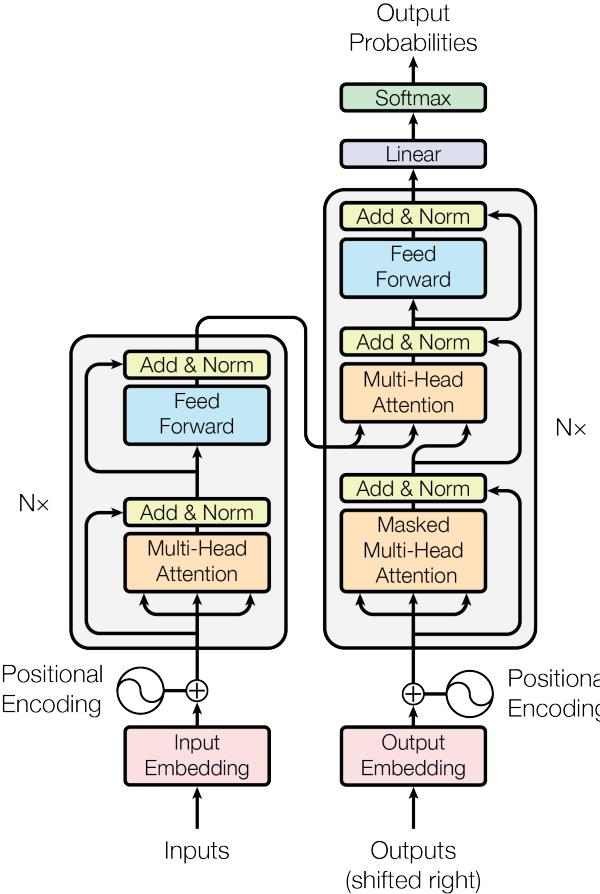
\includegraphics[width=\linewidth, height=0.75\textheight, keepaspectratio]{supplement/ee461f4421b4b3ee9ee47f2df3147cd6c5ea8ecec38495a9b419497230cdc1a3.jpg}
    \vspace{0.1em}
    {\footnotesize Figure: Visualizations of attention patterns from encoder layers.}
\end{column}
\end{columns}
\end{frame}



\section{Conclusion}



\begin{frame}{Summary}
    \begin{block}{The Transformer: A Paradigm Shift}
First sequence transduction model based \textbf{entirely} on attention mechanisms. Dispenses with recurrence and convolutions.
\end{block}

\begin{itemize}
    \item \textbf{Key Advantage:} Superior parallelization enables significantly faster training.
    \item Achieved new state-of-the-art results in machine translation (WMT 2014).
    \item Demonstrated strong generalization to other tasks (e.g., English constituency parsing).
    \item Core innovation: Multi-head self-attention for global dependencies.
    \item Architecture: Encoder-decoder stacks with residual connections and positional encoding.
\end{itemize}
\end{frame}
\begin{frame}{Future Work \& Impact}
    \begin{block}{Future Directions}
    \begin{itemize}
        \item Extend to other modalities: images, audio, video.
        \item Investigate local/restricted attention for very long sequences.
        \item Reduce sequential dependency in auto-regressive generation.
    \end{itemize}
\end{block}

\begin{block}{A Paradigm Shift}
    The Transformer dispenses with recurrence and convolution, establishing a new, parallelizable architecture for sequence modeling based \textbf{solely} on attention.
\end{block}

\begin{itemize}
    \item Opens the door for more efficient and powerful models.
    \item Sets a new state-of-the-art in machine translation.
    \item Demonstrates strong generalization to other tasks (e.g., parsing).
\end{itemize}
\end{frame}
\begin{frame}
    \centering
    \Huge \color{mathblue} Thank You!
\end{frame}\end{document}